\documentclass[letterpaper,11pt]{article}
\usepackage{amsmath}
\usepackage{tikz}
\usepackage{tabularx}
\usepackage{pgf-umlcd}
\renewcommand{\umlfillcolor}{white}
\renewcommand{\umldrawcolor}{black}
\usepackage[margin=1in,letterpaper]{geometry}
\usepackage{cite}
\usepackage[final]{hyperref}
\hypersetup{
	colorlinks=true
	linkcolor=blue,
	citecolor=blue,
	filecolor=magenta,
	urlcolor=blue         
}
\usepackage{blindtext}
\usepackage{listings}
\lstset{
  language=python, frame=single, numbers=left, breaklines=true
}
\usepackage{float}

\newcommand{\trivial}{$\mathcal{A}_T$\ }
\newcommand{\simple}{$\mathcal{A}_S$\ }
\newcommand{\improvedinc}{$\mathcal{A}_{II}$\ }
\newcommand{\dynamic}{$\mathcal{A}_{D}$\ }
\newcommand{\implicit}{$\mathcal{A}_{Impl}$\ }
\newcommand{\M}{$\mathcal{M}$}
\newcommand{\OD}{$\mathcal{O}(\Delta)$}
\newcommand{\ODM}{$\mathcal{O}(min\{\Delta, m^{2/3}\})$}
\begin{document}

\title{Seminar: Advances in Dynamic Algorithms \\ Maximal Independent Sets}
\author{Thilo Leon Fischer}
\date{\today}
\maketitle

\begin{abstract}
This report presents a performance comparison of different algorithms for
the dynamic maximal independent set problem. The evaluated algorithms
were created by Gupta et al. \cite{gupta2018simple} and Assadi et al.
\cite{assadi2019fully}. The algorithms were implemented in Python 3
and applied to datasets of varying size. The execution time for the
different algorithm update functions is measured and compared.

  % different algorithms to solve the maximal independent set problem
  % in a dynamic setting
\end{abstract}


\section{Introduction}
\label{sec:intro}

First, some basic definitions are made and the problem of maximal independent sets
is introduced.

A graph $G = (V, E)$ is a tuple consisting of a set of nodes $V$ and a set of
edges $E \subset V \times V$. The number of nodes is denoted by $n$, the number
of edges by $m$. The degree of a node $v$ is $deg(v)$. The maximum degree is
refered to by $\Delta$.

An independent set $IS$ is a subset of nodes with the property that no two nodes
in the $IS$ are neighbours, as formalised in equation \ref{eq:is}.

\begin{equation}
	\label{eq:is}
\forall u, v \in IS: {u, v} \notin E
\end{equation}

An independent set is considered maximal, if no node can be added to it without
violating the independent set property. A maximal independent set is abbreviated
as MIS in this report. A MIS is different from a maximum independent set, which
is an IS with the biggest possible size.

To compute a MIS for a given graph, it is possible to loop over all nodes and
consider a node to be in the MIS if no previous neighboring node is inside the
MIS. This approach has a complexity of $\mathcal{O}(m)$, and is denoted by the
symbol \trivial in this report.

However, in practice edges and nodes might be removed or added to the graph. In
this dynamic setting, the algorithm should calculate the set of nodes in the MIS
after each update. Executing the algorithm again after every update is not
optimal. Instead it is desirable to maintain information about the MIS across
updates to increase calculation speed.

Alternatively, this model can be relaxed to an implicit model. Then, the
algorithm is not required to maintain an explicit copy of the MIS. Instead it
implements a query system, where it answers whether a specific node is in the
MIS or not \cite{gupta2018simple}.

The next section \ref{Algorithms} presents several different algorithms to
compute a MIS. In section \ref{Implementation} details of the implementation are
discussed. The performance of these implementations is then evaluated in section
\ref{Evaluation}. Finally, a summary is contained in section \ref{Summary}.




% What is a graph?
% What is an IS?
% What is a MIS?

% What is the dynamic setting?
% What update is difficult?
% adjustement complexity
% amortized time per update
%

% \subsection[Resources]{Resources}
All code and files relevant to this report can be accessed at:
\newline
\url{https://www.github.com/thilofischer/dynamic\_mis}.

% The folder\textbf{dynamic_mis} contains the Python implementations for the algorithm discussed
% in section \ref{Algorithms}.

\section{Algorithms}
\label{Algorithms}

In this section several different algorithms will be presented to solve the MIS
problem in a dynamic setting. All algorithms that are discussed here use the
papers from Gupta et al. \cite{gupta2018simple} and Assadi et al.
\cite{assadi2019fully} as reference.

The first algorithm was already mentioned in the introduction \ref{sec:intro}.
It is the so called \textit{Trivial} \trivial algorithm.

% To adapt it to a dynamic setting,

After each update to the graph, the algorithm is executed again; It computes the
MIS from scratch for every update to the graph. This means that the time
complexity is $\mathcal{O}(m)$ and the adjustement complexity is
$\mathcal{O}(n)$.

The second algorithm is called the \textit{Simple} \simple algorithm. The
approach in this algorithm is to maintain a counter for each node. The values of
this counter represents how many of its neighbours are inside the MIS. If the
counter for a node is zero, then this node is inside the MIS. To keep this
counter value accurate, every node that leaves or enters the MIS has to inform
its neighbours so that they can update their counter value. Each update may
cause one node to leave the MIS and may cause up to $\Delta$ nodes to join the
MIS. These nodes also have to inform their neighbours. Overall the amortized
update time complexity is \OD.

Gupta et al. presented a slighty improved version of this \simple algorithm. In
this report it is refered to as the \textit{Improved Incremental} \improvedinc
algorithm. The difference to \simple is in the case of an edge insertion between
two nodes that are in the MIS. \simple does not specify which node should leave
the MIS. In \improvedinc, the node with lower degree is removed. This leads to
smaller number of neighbours that need to be informed about the state change.

The fourth algorithm \dynamic has a very fast amortized update time complexity
of \linebreak $\mathcal{O}(min\{\Delta, m^{2/3}\})$.
This is achieved by treating nodes differently based on their degree.
Heavy nodes are nodes with relatively many incident edges, while light nodes are
those with fewer neighbours.

The MIS is computed in two steps. In \simple a heavy nodes has to inform many
neighbours. For this reason, \dynamic only maintains a counter for light nodes.
The counter is maintained in the same way as in the \textit{Simple} algorithm.
At this stage the selected light nodes form an independent set but it may not be
maximal. So after every update, the \trivial algorithm is applied to the heavy
nodes that are not adjacent to a light node that is in the MIS.

The final algorithm \implicit operates in a different model than the previous
algorithms. Instead of maintaining an explicit copy of the MIS, only an
independent set is kept in memory. In this report this algorithm is called the
\textit{Implicit} algorithm. To get information about the MIS, the user of the
algorithm has to query the algorithm about the state of a specific node. Then
the algorithm checks whether the node is in the independent set or if it can be
added to it. Here, once again, nodes are differentiated by their degree.
\implicit maintains a counter only for heavy nodes. The dynamic calculation of
the count would be too slow for heavy nodes. For light nodes however, this
calculation can be done inside the query function, because they have few
neighbours.

In the implicit model not the amortized complexity is considered but the worst
case complexity. For \implicit the worst case complexity of updates and
queries is $\mathcal{O}(min(\Delta, \sqrt{m}))$.



% \subsection{Implicit Setting}
% In section \ref{sec:intro} the dynamic model was introduced, where
% the algorithm


\section{Implementation}
\label{Implementation}

The algorithms presented in the previous section were implemented using Python
3.8.2. To store and perform operations on graphs, the \textit{NetworkX} package
is used. To perform randomized operations, \textit{numpy.random} is used.

The strategy design pattern is applied to give all implementations a unified
interface. This interface is visualised in the UML diagram that can be seen in
figure \ref{fig:uml}.

%
% explain what each funciton does.
%

\begin{figure}[H]
  \begin{center}
  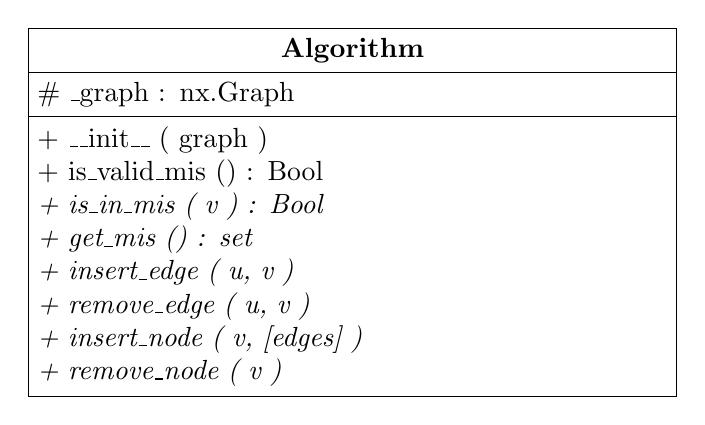
\begin{tikzpicture}
    \begin{class}[text width=8cm]{Algorithm}{0,0}
    \attribute {\# \_graph : nx.Graph}
    \operation {+ \_\_init\_\_ ( graph )}
    \operation {+ is\_valid\_mis () : Bool}
    \operation [0]{+ is\_in\_mis ( v ) : Bool}
    \operation [0]{+ get\_mis () : set}
    \operation [0]{+ insert\_edge ( u, v )}
    \operation [0]{+ remove\_edge ( u, v )}
    \operation [0]{+ insert\_node ( v, [edges] )}
    \operation [0]{+ remove\_node ( v )}
    \end{class}
  \end{tikzpicture}
  \end{center}
  \label{fig:uml}
  \caption{UML Class Diagram of the Algorithm interface}
\end{figure}

The \lstinline[]{__init__()} function takes a NetworkX graph as a parameter. In
this function the algorithms perform the operations to initialize their internal
data structures. The function \lstinline{is_valid_mis()} checks whether the MIS,
that the algorithm computed, is a valid MIS. This function should always return
\lstinline{True}. To access information about the MIS, the two functions
\lstinline{is_in_mis( v )} and \lstinline{get_mis()} can be used. The former
checks whether a given node is in the MIS, and the latter returns a set of all
nodes in the MIS. Note that these functions have side-effects in case the
\textit{Implicit} algorithm is used.

To perform an update, one of the four update functions can be used. When
inserting a node, edges to existing nodes can be passed along but are optional.

The different algorithms shown in section \ref{Algorithms} are implemented
as subclasses of \textit{Algorithm} and implement the six abstract functions.

% All implementations of a MIS algorithm can share
% To provide a unified interface to all algorithm implementations

\subsection{Testing}

To check that the implementation produces correct results, each algorithm was
tested. The relevant source code is located in the file
\textit{tests/test\_algorithm.py}.

To determine whether a set of nodes forms a MIS on a given graph, the function
\textit{Algorithm.is\_valid\_mis()} was implemented. In the testcases for this
function, an algorithm object was patched using the Python module
\textit{unittest.mock} to return pre-determined values as an answer. This was
done to produce valid and invalid maximal independent sets independently of any
specific implementation. The function is tested against four edge cases, three
of which expect the return value to be \textit{false}.

Using the \textit{Algorithm.is\_valid\_mis}, function the actual algorithm
implementations are tested.  To generate data for these testcases $G(n,
p)$-graphs were created. To make the testcases reproducible, fixed seeds are
used, so that every run of the testcase operates on the same graph.

For each algorithm four tests are performed.  These testcases correspond to the
four different updates: insert/remove node/edge.  Each testcase consists of a
loop that performs the updates until all nodes/edges are inserted or removed.
For the node insertion case, the starting graph is completely empty. For edge
insertions, the starting graph consists only of nodes.

After each update, it is verified that the set calculated by the algorithm is
actually a MIS, and that the update has been performed on the graph. For the
insertion testcases, after all updates have been performed the final graph is
compared against the original graph to check whether the resulting graph is the
desired graph.


\section{Evaluation}
\label{Evaluation}

To evaluate the performance of the different algorithms, the execution time of
multiple of updates is measured.
For this purpose five different datasets with varying size are used. 
The datasets are called:

\begin{enumerate}
  \itemsep 0em
  \item aves-wildbirds-networks \cite{wildbirds}
  \item topology \cite{konect:2016:topology, konect:zhang05, konect}
  \item facebook-wosn-links \cite{konect:2016:facebook-wosn-links, viswanath09, konect}
  \item youtube-u-growth \cite{konect:2016:youtube-u-growth, konect:mislove2, konect}
  \item brightkite \cite{konect:2016:loc-brightkite_edges, konect:cho2011, konect}
\end{enumerate}

The datasets 1-4 are used for edge insertion benchmarks, while dataset 5 is
used to evaluate edge deletion. The size of the datasets is shown in table \ref{tab:datasets}.

\begin{table}[h]
  \caption{Size of the datasets}
  \label{tab:datasets}
  \centering
  \setlength{\extrarowheight}{0.3em}
  \begin{tabular}{|c|c|c|c|c|c|}
    \hline
    Dataset & 1 & 2 & 3 & 4 & 5 \\
    \hline
    \hline
    Nodes & 202 & 34,761 & 63,731 & 3,223,589 & 52,228 \\
    \hline
    Edges & 11900 & 114,496 & 817,035 & 9,375,374 & 214,078 \\
    \hline
  \end{tabular}
\end{table}

One benchmark run consists of two parts. First is the initialization of the data
structures used by the algorithm. Here, the initial MIS is calculated for the
starting graph, with exception of the \textbf{ImplicitMIS} algorithm, which does
not keep an explicit copy of the MIS.

The second part of a benchmark run is a loop that calls an \textit{Algorithm}
function to perform an update. In listing \ref{lst:bench}, a code snippet of the
benchmarking code is shown.


\begin{lstlisting}[label={lst:bench}, caption=Benchmark Code Snippet]
def execute():
      algo = algo_cls(graph)
      for e in edges:
          algo.insert_edge(*e)

t = timeit.timeit(execute, number=1)
\end{lstlisting}

In order for the measured execution time to be reliable, five runs of a
benchmark are done. The results are then averaged. Averaging is chosen over a
boxplot, because the individual times only show very minor deviations.
For the detailed output, including the time of every single run, refer to the
files inside the \textbf{log/} folder in the repository.

Note that in listing \ref{lst:bench} on line 6 the number of runs is set to
one. Because the graph is modified during a run, a new graph instance needs to
be used for each run. However, the copy operations to create a new graph do not
depend on the algorithm under evaluation. So these operations should not
contribute to the run time of the algorithm, as they would only introduce more
unknown variables. Instead the \textit{timeit} function only performs one
benchmark run at a time and the code shown in listing \ref{lst:bench} is executed
five times to arrive at the final result.

\subsection{Results}

In this subsection, the results of the benchmark runs are presented. The
benchmarks were executed on an Intel Core i7-1065G7 with 16GB of memory. The two
updates that are benchmarked are edge insertions in section
\ref{sec:edgeinsertion} and edge deletions in section \ref{sec:edgedeletion}.


\subsubsection{Edge Insertions}
\label{sec:edgeinsertion}

In table \ref{tab:insertion} the average execution times are shown. The values
are the average over five runs in seconds. In case the execution took too long,
the table contains a \textbf{DNF}, denoting that the algorithm did not finish.
The threshold for this is 2 minutes. This cut-off was chosen to keep the time
required to perform five iterations of each algorithm manageable. One evaluation
of the \textit{Youtube} dataset for the three fastest algorithm takes over 20
minutes.


\begin{table}[H]
  \caption{Time for Edge Insertions}
  \label{tab:insertion}
  \centering
  \setlength{\extrarowheight}{0.3em}
  \begin{tabular}{|c|c|c|c|c|c|}
    \hline
    Data & Trivial \trivial & Simple \simple & Incremental \improvedinc & Dynamic \dynamic & Implicit \implicit \\
    \hline
    \hline
    Wildbirds & 1.281 & 0.013 & 0.012 & 0.064 & 0.020 \\
    \hline
    Topology & DNF & 0.430 & 0.504 & 3.205 & 0.696 \\
    \hline
    Facebook & DNF & 2.582 & 2.228 & DNF & 4.042 \\
    \hline
    Youtube & DNF & 67.058 & 60.695 & DNF & 95.488 \\
    \hline
  \end{tabular}
\end{table}

First note the execution times for the \textit{Trivial} algorithm.
It is considerably slower than the other algorithms on the smallest dataset.
And for the next biggest dataset it does not compute the result in 2 minutes.
This clearly demonstrates the need for a dynamic approach to solve the MIS
problem in an environment with many updates.

Now compare the execution times of all algorithms on the \textit{Wildbirds}
dataset. \textit{Simple} is the second fastest after the improved version of it,
the \textit{Improved Incremental} algorithm. It makes a better choice for removing
a node from the MIS for the cost of an additional degree comparison.
In the largest dataset, the improvement to the \textit{Simple} algorithm
manifest in an improvement of \~9\%, when comparing the \textit{Improved Incremental}
to the \textit{Simple} algorithm.

The \textit{Dynamic} algorithm presented in \cite{gupta2018simple} performs
worse than the simpler algorithms. Profiling the code did not reveal
any obvious bottlenecks for this algorithm.
However, inspecting the datasets showed that in the \textit{Youtube} dataset
only six nodes are considered heavy in the full dataset. In the complete graph
of the \textit{Facebook} dataset no nodes are heavy. The same is true for the
\textit{Wildbirds} network. In the \textit{Topology} dataset three nodes are
heavy in the full graph.
Although it is not as severe, the \textit{Implicit} algorithm is also slower.

Thus it is likely that for these specific datasets, the more sophisticated
algorithms can not realize their full potential.
In the contrary, the more complex code adds overhead and slows the execution down.

% Rather the more complex code adds overhead that does not help to speed the execution
% up because it is only applicable for heavy nodes.

% Rather the higher complexity of the code added overhead, that slowed them down.

% Thus it is likely that this difference is caused by the more complicated
% implementation. This factor is not accounted for when considering the asymptotic
% complexity is evaluated.

A case where this became obvious occured during the implementation of the
\textit{ImprovedIncremental} algorithm. It is almost identical to the
\textit{Simple} algorithm. Thus the first implementation used inheritance. This
approach is shown in listing \ref{lst:slowinc}. However the additional
\lstinline[]{if}-statement and function call negated the speed improvement from
differentiating between the lower and higher degree node. The algorithm that is
faster in theory was actually slower in practice.

\begin{lstlisting}[label={lst:slowinc}, caption={Slow implementation}]
class ImprovedIncrementalMIS(SimpleMIS):
  def insert_edge(self, u, v):
    lower_deg, higher_deg = (u, v) if self._graph.degree(u) < self._graph.degree(v) else (v, u)
    SimpleMIS.insert_edge(self, lower_deg, higher_deg)
\end{lstlisting}

Instead it is faster to inline the code from \textit{Simple}. This inlined implementation was used for the benchmarks. And an improvement can be seen in three
of the four datasets.

% Theoretical does not matter as much for fast code
% comparison  between Simple and incremental

\subsubsection{Edge Deletions}
\label{sec:edgedeletion}

To evaluate the performance of edge deletions, the \textit{Brightkite}
\cite{konect:2016:loc-brightkite_edges, konect:cho2011, konect} dataset is used.

The edges to be removed were chosen randomly but in a reproducible way. So every
benchmark run performs exactly the same operations. The first benchmark removes
1,000 edges, the second 10,000, the third removes 100,000 edges. For edge
deletions, the \textit{Improved Incremental} algorithm is not used, because it
only supports incremental updates. For deletions, it is identical to the
\textit{Simple} algorithm.

\begin{table}[h]
  \caption{Time for Edge Deletions}
  \label{tab:deletion}
  \centering
  \setlength{\extrarowheight}{0.3em}
	\begin{tabular}{|c|c|c|c|c|c|}
		\hline
		Removals & Trivial \trivial & Simple \simple & Dynamic \dynamic & Implicit \implicit \\
		\hline
		\hline
		% 1000 & 2.68 & 0.018 & 0.017 & 0.029 \\
		1000 & 77.246 & 0.136 & 0.158 & 0.100 \\ % the initialisation takes 0.153
		\hline
		10,000 & DNF & 0.157 & 0.266 & 0.166 \\
		\hline
		100,000 & DNF & 0.361 & 1.252 & 0.793 \\
		\hline
	\end{tabular}
\end{table}

In this scenario \textit{Trivial} performs even worse than in the insertion
benchmark in the previous section. While the three more sophisticated approaches are fairly evenly matched
for few updates. When stepping up from 1,000 deletions to 10,000, the execution
time does not increase very much. This is caused by the slow initialization
phase. In the insertion case, the initial graph consists only of nodes without
their edges. So the initialization is basically a loop that adds all nodes to
the MIS, and thus is relatively fast. However, in the deletion case, the initial
graph is the full dataset. As shown in figure \ref{tab:datasets}, the brightkite
dataset has 52,228 nodes and 214,078 edges.

To initialize, \simple performs a single execution of the
\trivial algorithm. This alone takes ca. 0.140 seconds, 89\% of the
runtime for 10,000 updates. When only few updates are performed, the
\textit{Implicit} algorithm benefits from the low initialisation overhead.
Again, the \textit{Dynamic} algorithm from \cite{gupta2018simple}, is the
slowest. In theory, the \textit{Dynamic} algorithm is faster by treating nodes
differently based on their degree. However, after performing the benchmark,
inspection showed, that in this dataset no node is considered to be heavy.
A similar observation as for the datasets 1-4.


% nicht 10mal solange wegen der langen initialization


% \subsection{What I learned}

\section{Summary}
\label{Summary}

In this paper five different algorithms to solve the dynamic MIS problem
were evaluated on five datasets. Each of these algorithms belongs to a different
complexity class.
The \textit{Trivial} algorithm perfomed very poorly compared to the other algorithms.
This demonstrated that applying a static algorithm to a dynamic use case
does not yield acceptable results.
Also the \dynamic and \implicit algorithm did not perform as expected. They were
slower, in some cases by orders of magnitude, than their more simple counterparts.
However, this observation might be caused by the specific datasets that were employed
for the benchmarking. \dynamic and \implicit have a lower amortized complexity because
they treat nodes with a high degree differently. The threshold for a node to be
considered heavy is so high that, for these datasets, no improvement could
be observed. Rather the more complex code added overhead which slowed the execution
down.

A conclusion from this observed behavior could be that when chosing an algorithm in practice,
not only should the theoretical complexity be a factor but also the data it will
operate on. And whether the algorithm is suited for the specific kind of data.



\bibliography{report}{}
\bibliographystyle{plain}

\end{document}

